\chapter{Review Of Literature} % Main chapter title

\label{Chapter2} % Change X to a consecutive number; for referencing this chapter elsewhere, use \ref{ChapterX}

\lhead{Chapter 2. \emph{Background}}
\label{sec:2}
\section{Introduction To Machine Learning}
Machine Learning (ML) is the sub-field of the much broader concept of Artificial Intelligence. The primary goal of ML, applied to the problem of interest here, is to understand and develop correlations within a given data, which improve automatically through experience. Specifically, these correlations (or mathematical models) are not prescribed \textit{a priori} and are developed by the ML algorithms via analysis of the input data. In classical computing, most algorithms are sets of programmed instructions which the computers use to calculate or solve the problem. ML algorithms on the other hand enable a computer to train on input data and output values that lie within an acceptable range using statistical analysis. Machine learning finds extensive use in many present day technologies. Some real world applications are shown in Figure \ref{fig:app-ml}. 

\begin{figure}[!h]
	\centering
	\includegraphics[width=0.7\textwidth]{applications-of-machine-learning.png}
	\hspace{1mm}
	\caption{Various applications of machine learning \cite{mlimage}.} 
	\label{fig:app-ml}
\end{figure}

Deep Learning is a branch of machine learning which is completely based on artificial neural networks. An artificial neural network (ANN) is a flexible mathematical structure which is capable of identifying complex nonlinear relationships between input and output data sets.  It achieves great flexibility and power by learning to represent the world as a nested hierarchy of concepts, with each concept defined in relation to simpler concepts, and more abstract representation computed in terms of less abstract ones \cite{dlintro}. A number of deep learning architectures such as deep neural networks, deep belief networks, recurrent neural networks and convolutional neural networks have been applied to fields including computer vision, speech recognition, natural language processing and audio recognition. These networks have produced results comparable to and in some cases surpassing human expertise. In this thesis, we have employed deep neural networks and recurrent neural networks to develop a model for predicting the deformation behavior.

\section{Deep Learning}
In this section, we describe the fundamentals of neural networks.

\subsection{The Neuron}
A neuron is a fundamental unit of the human brain. The core functionality of a neuron is to input information from other neurons, process it and pass on the results to other cells. It receives information from different connections, which are dynamically strengthened or weakened based on how often it is used (learning new concepts) and this strength determines the effect of the input on the output. Once the inputs are weighted by the strength of their connections, they are summed and transferred to the next neuron. This concept of a neuron can be easily represented on a computer. An artificial neuron has the capability to take in inputs, $x_i, i \in 1,N$ (for $N$ neurons), which are multiplied by their respective weights, $w_i$, and then summed to produce the output or logit of that neuron which can be given as: 
\begin{equation}
z = \sum_{i=1}^{i=n} w_ix_i
\end{equation}

A constant may be added to this logit and then passed through a function $f$ to produce the output $y = f(z)$. The function, $f$, is called the activation function and introduces non-linear behavior in the neuron. Alternatively, the logic may be expressed as a dot product between two vectors, $\boldsymbol{x} = [x_1, x_2,...,x_n]$ as the input vector and $\boldsymbol{w} = [w_1, w_2,...,w_n]$ \cite{buduma2017fundamentals}. The expression thus becomes:
\begin{equation}
y = f(\boldsymbol{w}\cdot\boldsymbol{x} + b)
\end{equation}

\begin{figure}[!h]
	\centering
	\includegraphics[width=1.0\textwidth]{Pictures/hdnnfin.png}
	\hspace{1mm}
	\caption{Schematic of a neuron.} 
	\label{fig:neuron}
\end{figure}

\subsection{Artificial Neural Network}
A single neuron may not be sufficient to solve or model complicated problems. Analogous to our brain, which is made up of millions of neurons arranged in multiple layers, we can construct an artificial neural network. A neural network consists of a number of neuron hooked to each other. The first layer of nodes receives the input data (input layer) and the last layer's output  (output layer) is the final answer computed by the neural network.  All the layers in between are called the hidden layers. The weight of the connection between the $i^{th}$ neuron in the $k^{th}$ layer with $j^{th}$ neuron in the $(k+1)^{th}$ layer is represented by $w_{i,j}^{(k)}$. Our network's ability to solve problems, is dependent upon finding an optimal value of these weights \cite{buduma2017fundamentals}. Some important aspects of neural networks are as follows:

\begin{enumerate}
\item	Neurons in the same layer have no connections between them and no data is transmitted from a higher layer to a lower layer.
\item	It is not necessary for all the layers to have the same number of neurons.
\item	All the neurons may not have their outputs connected to all the neurons in the next layer. Some connections are dropped to optimize the network and the training process.
\item The input and outputs are vectorized representations.
\end{enumerate}

\begin{figure}[!h]
	\centering
	\includegraphics[width=0.45\textwidth]{Pictures/hdaannnpng.png}
	\hspace{1mm}
	\caption{Schematic of a simple neural network.} 
	\label{fig:nn}
\end{figure}

Figure \ref{fig:nn} shows a simple neural network with 3 layers (input layer, 1 hidden layer and output layer) and 3 neurons in each layer. Mathematically, neural networks can be represented as a series of vector and matrix multiplications. Let us say $\boldsymbol{x} = [x_1, x_2,...,x_n]$ is the input to the $i^{th}$ layer, which propagates the output $\boldsymbol{y} = [y_1, y_2,...,y_m]$. We can represent the weights of connections in the form of a weight matrix $\boldsymbol{W}$ of size $m\times n$ along with a bias vector $\boldsymbol{b}$. Then the following holds true:

\begin{equation}
\boldsymbol{y} = f(\boldsymbol{W}^T\boldsymbol{x} + \boldsymbol{b})
\end{equation}

A single neural network can consist of different neurons stacked together in different layers. The activation function, $f$, a neuron applied to their logit, $z$, decides the type of neuron it is. For example, a linear neuron may be of the form: $f(z) = az + b$. A linear neuron is easily computed, but runs into a number of limitations. A network with only linear neurons can mathematically be expressed as a network without hidden layers \cite{buduma2017fundamentals}. Therefore, in order to learn complex relationships we need an activation function which can employ some non-linearity. To help achieve this, there exist 3 major types of neurons. The first one is the sigmoid neuron:

\begin{equation}
f(z) = \frac{1}{1+e^{-z}}
\end{equation}

From the equation above, we can see that for very small logit values the output of the function is close to 0. While for large values of the logit, the output is close to 1. Between 0 and 1, the outputs are as shown in the Figure \ref{fig:sigmoid}.

\begin{figure}[!h]
	\centering
	\includegraphics[width=0.7\textwidth]{sigmoid-big.eps}
	\hspace{1mm}
	\caption{Output of sigmoid neuron as a function of z.} 
	\label{fig:sigmoid}
\end{figure}

Another kind of neuron is the tanh neuron, which also uses a similar S-shaped curve but with values ranging from -1 to 1. This is unlike the sigmoid function where values are between 0 and 1. The function is, as expected, $f(z) = tanh(z)$. The relationship between the input logits and output values can be seen in Figure \ref{fig:tanh}.

\begin{figure}[!h]
	\centering
	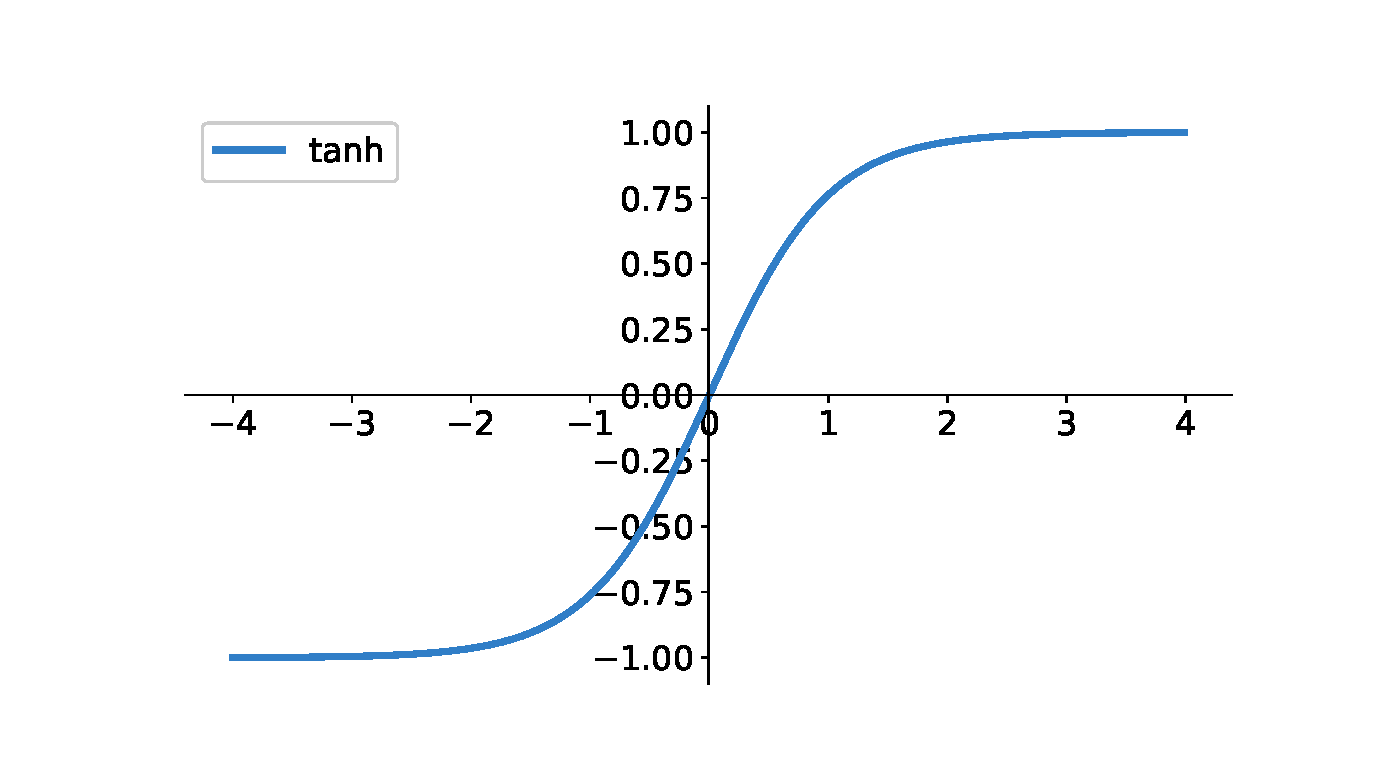
\includegraphics[width=0.7\textwidth]{tanh-big.eps}
	\hspace{1mm}
	\caption{Output of tanh neuron as a function of z.} 
	\label{fig:tanh}
\end{figure}

The last type of neuron we are going to discuss is the restricted linear unit (ReLU) neuron. This function is given by $f(z) = max(0,z)$ resulting in the graph shown in Figure \ref{fig:relu}.

\begin{figure}[!h]
	\centering
	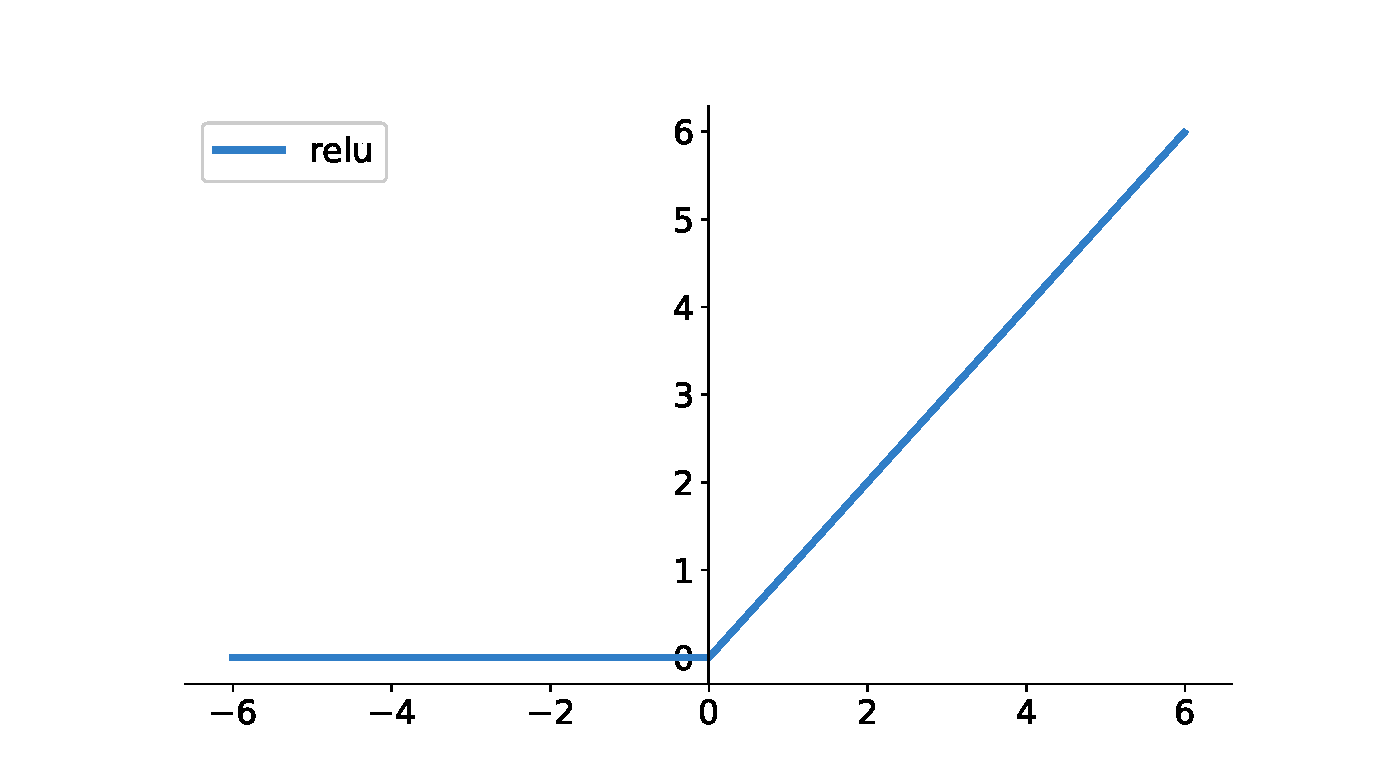
\includegraphics[width=0.7\textwidth]{relu-big.eps}
	\hspace{1mm}
	\caption{Output of ReLU neuron as a function of z.} 
	\label{fig:relu}
\end{figure}

Other activation functions also exist, for example, like exponential linear unit (ELU), binary step, SoftPlus, Leaky ReLU \cite{karlik2011performance}. The ones described in this report are the most commonly used.

\subsection{Training}
A deep learning neural network learns to map a set of inputs to outputs from training data. As there are a large number of unknowns, we cannot calculate the perfect set of weights for the network. Instead, training a neural network is treated as an optimization problem and an algorithm is used to find a set of weights which make relatively good predictions. Before an optimization algorithm is employed we need a metric to measure how well the weights are doing at every step and updating them accordingly. This metric is our loss function and the goal of the training process is to minimize this loss function. There is no one loss function which can be used for all machine learning problems. Choice of the loss function depends primarily on the type of algorithm we are using and the ease with which the function's derivative can be calculated \cite{whytrain}. 

There are two major types of loss functions: regression losses, and classification losses \cite{losses}. In regression, the model deals with predicting a continuous variable like stress, strain for a particular grain. Classification, on the other hand deals with predicting the output from a set of finite categorical value, example labeling a grain as a hotspot. A detailed description of loss functions are given below:

\begin{enumerate}
\item	\textbf{Mean Square Error (MSE)}: is computed from the average of squared difference between actual observations and predictions. The squaring enables heavy penalization of predictions that are far away from the true value. MSE has favorable mathematical properties  of convexity, symmetry, and differentiability. Minimising MSE often has a closed-form analytical solution, and when they do not, iterative numerical optimization procedures are often easy to formulate, since the gradient is easy to compute \cite{4775883}. If $y_i$ is the true value and $\hat{y_i}$ is the predicted value then it can be calculated as: 
\begin{equation}
MSE = \frac{\sum_{i=1}^{n}\left(y_i - \hat{y_i}\right)^2}{n}
\end{equation}
\item	\textbf{Mean Absolute Error (MAE)}: is computed as the averaged sum of absolute difference between actual observations and predictions. However MAE, has proved to under-fit training date due to it's low variance over data points \cite{wang2020imae}. It is given by:
\begin{equation}
MAE = \frac{\sum_{i=1}^n|y_i - \hat{y_i}|}{n}
\end{equation}
\item \textbf{Cross Entropy Loss}: is commonly used for classifications problems. Cross-entropy loss increases as the predicted probability diverges from the actual label. The mathematical formulation is given as: 
\begin{equation}
Cross Entropy Loss = -(y_ilog(\hat{y_i}) + (1-y_i)log(1-\hat{y_i}))
\end{equation}
\end{enumerate}

Having described the loss functions, we now describe an algorithm to find the weights and biases so that the network's output approximates well for all training inputs. We start with looking at a simpler version of the mean squared error cost function and later generalize for a neural network. The cost function can be written as follows:
\begin{equation}
C(\boldsymbol{w},\boldsymbol{b}) = \frac{\displaystyle\sum\limits_x ||y(x) - a||^2}{n}
\end{equation}
Here, $\boldsymbol{w}$ and $\boldsymbol{b}$ denote the weights and biases respectively, $n$ is the number of training inputs and $a$ is the output from the network. The aim of the optimization algorithm is to minimise this cost function: the training algorithm has done well if it can find weights and biases such that $C(\boldsymbol{w},\boldsymbol{b})\approx 0$. To achieve this we use a gradient descent algorithm. Currently the problem looks very complicated - the interpretation of $\boldsymbol{w}$ and $\boldsymbol{b}$ and the summation function in the background. Let us ignore most of these structures and just concentrate on the minimization aspect. Let us further assume that we have a function of two variables $w_1$ and $w_2$, and we want to minimise this function. So our new function is $C(w_1, w_2)$, and for small changes $\Delta w_1$, $\Delta w_2$ the corresponding change in $C(w_1, w_2)$ can be given as:
\begin{equation}
\Delta C \approx \frac{\partial C}{\partial w_1}\Delta w_1 + \frac{\partial C}{\partial w_2}\Delta w_2
\end{equation}
We can define vector as $\boldsymbol\Delta w = (\Delta w_1, \Delta w_2)^T$ and the gradient vector by $\boldsymbol\nabla C$. The gradient vector, $\boldsymbol\nabla C$, is the direction of steepest descent for any function, hence we move along this direction.
\begin{equation}
\boldsymbol{\nabla C} = \left(\frac{\partial C}{\partial w_1}, \frac{\partial C}{\partial w_2}\right)^T
\end{equation}
With these definitions, Equation 2.9 can be written as
\begin{equation}
\Delta C \approx \boldsymbol{\nabla C}\cdot \boldsymbol \Delta w
\end{equation}
We want $\Delta C$ to always be negative because we want to minimise the function. We can choose our $\Delta v$ such that $\Delta C$ is always negative. \cite{nielsen2015neural}
\begin{equation}
\boldsymbol\Delta w = -\eta\boldsymbol\nabla C
\end{equation}
$\eta$ is a small positive character known as the learning rate. It is a hyperparameter that controls how much one should adjust the model in response to the estimated error everytime the weights are updated. Very small a value may cause results in a long training process, whereas a large value may always yield a sub-optimal set of weights and never converge \cite{learningrate}. Selection of learning rate is also another crucial step in the training process. Moving on, from Equation 2.11 we can say $\Delta C \approx -\eta\boldsymbol\nabla C\cdot \boldsymbol\nabla C = -\eta||\boldsymbol\nabla C||^2$. As $||\boldsymbol\nabla C||^2 \geq 0$, this guarantees that $\Delta C \leq 0$, i.e., $C$ will always decrease. Thus, the weights can be updated using the following rule:
\begin{equation}
\boldsymbol w \rightarrow \boldsymbol w^{'} = \boldsymbol w - \eta\boldsymbol\nabla C
\end{equation} 

\begin{figure}[!h]
	\centering
	\includegraphics[width=0.6\textwidth]{2-var-grad.png}
	\hspace{1mm}
	\caption{Error surface as a function of $w_1$ and $w_1$} 
	\label{fig:err-surf}
\end{figure}
The above example as we spoke earlier is a very simplified case with just two weights taken into consideration. But actual neural networks have a large number of weights and biases segregates into different layers. We need a systematic algorithm to update all the values according to the error. Back-propagation helps in understanding how changing the weights and biases changes the cost function. Before we get started let us define some notations: $w_{jk}^l$ denotes the weight for the connection from $k^{th}$ neuron in the $(l-1)^{th}$ layer to the $j^{th}$ neuron in the $l^{th}$ layer. Similarly for biases, $b_j^l$ for the bias of $j^{th}$ neuron in the $l^{th}$ layer. $a_j^l$ will be used for the activation. $L$ denotes the last layer in the network. The goal of back-propagation is to compute partial derivatives, $\partial C/\partial w$ and $\partial C/\partial b$, with respect to any weight or bias. Let us say we introduce an error $\Delta z_j^l$ in the logit of the $j^{th}$ neuron in the layer $l$. This will change the output give by this neuron's activation function and propagate through the later layers finally cost function to change by $\frac{\partial C}{\partial z_j^l}\Delta z_j^l$. Thus in some sense we can define the error in that neuron by
\begin{equation}
\delta_j^l = \frac{\partial C}{\partial z_j^l}
\end{equation}
$\boldsymbol{\delta^l}$ will denote the vector of errors assiciated with layer $l$. Using backpropagation we will be able to calculate $\boldsymbol{\delta^l}$ for all the layers and relates those to our variables of interest through, $\partial C/\partial w_{jk}^{l}$ and $\partial C/\partial b_j^l$. The backpropagation algorithm is based on four fundamental equations which give us a way of computing both the gradient of the cost function and error $\boldsymbol{\delta^l}$ \cite{nielsen2015neural}.
\begin{enumerate}
\item \textbf{Error in output layers}: is given below. The $\partial C/\partial a_j^L$ measures how fast the cost function changes with the activation of the $j^{th}$ neuron in the output layer. The second term accounts for changes in the activation function $\sigma$ with changes in $z_j^L$.
\begin{equation}
\delta_j^l = \frac{\partial C}{\partial a_j^L}\sigma^{\prime}(z_j^L)
\end{equation}
The equation can be re-written for all neurons using matrix-based form using  Hadamard product, which is basically the element-wise product of two vectors.
\begin{equation}
\boldsymbol{\delta^L} = \nabla_a C \odot \sigma^{\prime}(z^L)
\end{equation}
\item \textbf{Error in terms of error in the next layer}: is given below where $(w^{l+1})$ is the weight matrix for the $(l+1)^{th}$ layer. If we know the error $\boldsymbol{\delta^{l+1}}$ for $(l+1)^{th}$ layer, then by mutiplying the transpose of the weight matrix we move the error backward through the network to give us the measure of error at the $l^{th}$ layer. By taking the Hadamard product with $\sigma^{\prime}(z^L)$ the error moves backward through the activation layer, giving us $\boldsymbol{\delta^l}$ for that layer.
\begin{equation}
\boldsymbol{\delta^l} = ((w^{l+1})^T \delta^{l+1})\odot \sigma^{\prime}(z^l)
\end{equation}
Using the equations above, we can calcualte the $\boldsymbol{\delta^l}$ for any layer starting with the output layer. 
\item \textbf{Change of error with bias}: is a simple equation given by:
\begin{equation}
\frac{\partial C}{\partial b_j^l} = \delta_j^l
\end{equation}
\item \textbf{Change of cost with any weight}: can now easily be given by the following equation. We already know how to compute $\boldsymbol{a^{l-1}}$ and $\boldsymbol{\delta^l}$.
\begin{equation}
\frac{\partial C}{\partial w_{jk}^l} = a^{l-1}_k \delta^l_j
\end{equation}
\end{enumerate}

\subsection{Recurrent Neural Networks}
Recurrent Neural Networks (RNNs) have played an important role in the field of machine learning ever since their introduction and development in the 1990s. They are used to learn time-varying and sequential patterns. \cite{medsker2001recurrent} RNNs leverage a special type of neural layer, known as recurrent layers which makes different from a neural network. The recurrent layer enables the network to maintain state between the uses of the network. All the neurons in an RNN have three types of connections: (i) incoming connections from the neuron of the previous layer (input) (ii) outgoing connections leading to neurons in the next layer (output), and (iii) recurrent connections between neurons in the same layer. Thus, a fully connected recurrent layer has information flowing from every neuron to every other neuron in the same as well as the next layer (including itself). A recurrent layer with $r$ neurons has $r^2$ connections within the same layer.
\begin{figure}[!h]
	\centering
	\includegraphics[width=0.6\textwidth]{Pictures/rnn-layer.png}
	\hspace{1mm}
	\caption{A recurrent layer with connections between neurons in the same layer. } 
	\label{fig:err-surf}
\end{figure}

RNNs are a category of neural networks where output from the previous time steps is taken as input for the current time-step. A RNN instance can actually be expressed as a feed forward neural network for a given fixed lifetime ($t$ time-steps). This transformation is referred to as "unrolling" the RNN through time. The update graph formed by unrolling is a useful way to visualise RNNs. The transformation is performed by repeating the neurons in the recurrent layer $t$ times, once for each time-step. Similarily the input and output connections are redrawn as they were in the original network and all the feed forward connections are made. Finally, feed forwards connections are drawn from each time-step replica to the next time-step as recurrent neural networks use neuronal activation from the previous time-step. Consider an input with $T$ timesteps, $I$ input units, $H$ hidden units, and $K$ output units. Let $x_i^t$ be the input $i$ at time $t$, $z_j^t$ be the input logit at of unit $j$ and $y_j^t$ be the activation. Then for hidden units, the logit can be written as
\begin{equation}
z_h^t = \sum_{i=1}^{I} w_{ih}x_i^t + \sum_{h^\prime =1}^H w_{h^\prime h}y_{h^\prime}^{t-1}
\end{equation}
\begin{figure}[!h]
	\centering
	\includegraphics[width=0.85\textwidth]{Pictures/unrolled-rnn.png}
	\hspace{1mm}
	\caption{RNN unrolled over time} 
	\label{fig:err-surf}
\end{figure}

The unrolled RNN can be trained by computing the gradient and using the techniques used for a feed forward neural network. However, for standards RNN architectures the range of context that can be accessed is quite limited. The influence of the inputs on the hidden layers either decays or blows exponentially as it cycles around the network's recurrent connections. This is often referred to as the problem of vanishing gradient \cite{hochreiter1998vanishing}. It is depicted in the figure given below. The shade of the node in the unrolled RNN indicates the relevance of the input at the first time step (darker the shade, greater the sensitivity). Numerous attempts were made to solve this problem, one of which is long short-term memory networks. 
\begin{figure}[!h]
	\centering
	\includegraphics[width=0.85\textwidth]{Pictures/vanishing-grad.png}
	\hspace{1mm}
	\caption{Vanishing gradient.} 
	\label{fig:err-surf}
\end{figure}

\subsection{Long Short-Term Memory (LSTM) Networks}
Long short-term memory networks were introduced by Hochreiter and Schmidhuber with the basic principle that the network would be designed for transmitting useful information multiple time-steps into the future  \cite{hochreiter1997long}. The LSTM architecture consists of memory cells, which are recurrently connected sub-nets. This memory cell is responsible for holding important information that the network has learnt over time and the network is designed to maintain this information with time. The memory cell functions with the help of three gates, which are discussed next. The schematic of a LSTM unit \hat{y_i} can be seen in figure-\ref{fig:lstm-cell}.
\begin{figure}[!h]
	\centering
	\includegraphics[width=0.85\textwidth]{Pictures/lstm-cell.png}
	\hspace{1mm}
	\caption{A LSTM unit.} 
	\label{fig:lstm-cell}
\end{figure}

The memory cells have a keep gate, shown in figure-\ref{fig:keep-gate}, which determines how much of the previous memory is useful and will be stored for future use. Memory state from the previous time-step is stored in the form of a tensor, rich in information. To figure out the elements in the memory tensor which are still useful, a bit tensor (tensor of zeros and ones) is calculated that we multiply to the memory state tensor. Intuitively, a zero means that the element's information is useless and one means that it is useful. The bit tensor is approximated by concatenating the output from the previous time-step along with the input of this time-step and applying a sigmoidal activation to them. The sigmoid function outputs value very close to 1 or 0 and hence works well for this task. 
\begin{figure}[!h]
	\centering
	\includegraphics[width=0.85\textwidth]{Pictures/keep-gate.png}
	\hspace{1mm}
	\caption{Architecture of the keep gate of the LSTM unit.} 
	\label{fig:keep-gate}
\end{figure}

Once the LSTM knows which information is useful, it is ready to write into the memory state, shown in figure-\ref{fig:write-gate}. This part is handled by another LSTM unit called the write gate. The write gate's function can be broken down into two major parts. Figuring out what information to write into the state is the first step. This is computed by concatenating the output from the previous time-step along with the input of this time-step and applying a tanh activation to them. The second part involves figuring part which parts are relevant and need to be stored in the new state. A similar strategy is used as the keep gate by creating a bit vector and multiplying it with the intermediate tensor. The result is added with the output of the keep gate to create a new state. 
\begin{figure}[!h]
	\centering
	\includegraphics[width=0.85\textwidth]{Pictures/write-gate.png}
	\hspace{1mm}
	\caption{Architecture of the write gate of the LSTM unit } 
	\label{fig:write-gate}
\end{figure}

At the final step, the LSTM unit provide it's output. The structure of the output gate, shown in figure-\ref{fig:output-gate}, is similar to the write gate. Tanh activation is applied to the state vector to form an intermediate tensor. A sigmoidal layer is used to create the mask using the current input and previous output. The intermediate tensor is multiplied by the bit tensor(mask) to produce the final output.
\begin{figure}[!h]
	\centering
	\includegraphics[width=0.85\textwidth]{Pictures/output-gate.png}
	\hspace{1mm}
	\caption{Architecture of the output gate of the LSTM unit.} 
	\label{fig:output-gate}
\end{figure}

The key equations involved in LSTM are given below where $\odot$ represents the Hadamard product, tanh is applied element-wise, $x_t, c_t$ and $h_t$ are the input, memory cell status and output of the LSTM at time $t$. $i_t, o_t$ and $k_t$ are the functional values of the write, output and keep gate. $W$s denote the weight matrix between the input and the gate and $b$s are the biases. 
\begin{equation}
    i_t = \sigma \left(W_{xi}x_t + W_{hi}h_{t-1} + W_{ci}\odot c_{t-1} + b_i \right) 
\end{equation}
\begin{equation}
    k_t = \sigma \left(W_{xk}x_t + W_{hk}h_{t-1} + W_{ck}\odot c_{t-1} + b_k \right)
\end{equation}
\begin{equation}
    c_t = f_t\odot c_{t-1} + tanh\left(W_{xc}x_t + W_{hc}h_{t-1} + b_c \right)
\end{equation}
\begin{equation}
    o_t = \sigma \left(W_{xo}x_t + W_{ho}h_{t-1} + W_{co}\odot c_{t-1} + b_o \right)
\end{equation}
\begin{equation}
    h_t = o_t\odot tanh(c_t)
\end{equation}